% IEEE standard conference template; to be used with:
%   spconf.sty  - LaTeX style file, and
%   IEEEbib.bst - IEEE bibliography style file.
% --------------------------------------------------------------------------

\documentclass[letterpaper]{article}

\usepackage{spconf,amsmath,amssymb,graphicx,hyperref,subcaption}
\usepackage{algorithm,algpseudocode} %algorithmicx

% |X|
\newcommand{\abs}[1]{\left| #1 \right|}
%keywords
\newcommand{\kif}[0]{\textbf{if}\hspace{1mm}}
\newcommand{\kthen}[0]{\textbf{then}\hspace{1mm}}
\newcommand{\kand}[0]{\hspace{1mm}\textbf{and}\hspace{1mm}}
% bold paragraph titles
\newcommand{\mypar}[1]{{\bf #1.}}

% Title.
% ------
%% TODO
\title{Something with connected components}
%
% Single address.
% ---------------
\name{Michael Bernasconi, Roman Haag, Giovanni Balduzzi, Lea Fritschi}
\address{Department of Computer Science\\ ETH Z\"urich\\Z\"urich, Switzerland}

% For example:
% ------------
%\address{School\\
%		 Department\\
%		 Address}
%
% Two addresses (uncomment and modify for two-address case).
% ----------------------------------------------------------
%\twoauthors
%  {A. Author-one, B. Author-two\sthanks{Thanks to XYZ agency for funding.}}
%		 {School A-B\\
%		 Department A-B\\
%		 Address A-B}
%  {C. Author-three, D. Author-four\sthanks{The fourth author performed the work
%		 while at ...}}
%		 {School C-D\\
%		 Department C-D\\
%		 Address C-D}
%

\begin{document}
%\ninept
%
\maketitle

%The hard page limit is 6 pages in this style. Do not reduce font size
%or use other tricks to squeeze. This pdf is formatted in the American letter format, so the spacing may look a bit strange when printed out.

\begin{abstract}
%Describe in concise words what you do, why you do it (not necessarily
%in this order), and the main result.  The abstract has to be
%self-contained and readable for a person in the general area. You
%should write the abstract last.
\end{abstract}

\section{Introduction}\label{sec:intro}

%Do not start the introduction with the abstract or a slightly modified
%version. It follows a possible structure of the introduction.
%Note that the structure can be modified, but the
%content should be the same. Introduction and abstract should fill at most the first page, better less.

\mypar{Motivation}
%The first task is to motivate what you do.  You can
%start general and zoom in one the specific problem you consider.  In
%the process you should have explained to the reader: what you are doing,
%why you are doing, why it is important (order is usually reversed).

%For example, if my result is the fastest sorting implementation ever, one
%could roughly go as follows. First explain why sorting is important
%(used everywhere with a few examples) and why performance matters (large datasets,
%realtime). Then explain that fast implementations are very hard and
%expensive to get (memory hierarchy, vector, parallel).

%Now you state what you do in this paper. In our example:
%presenting a sorting implementation that is
%faster for some sizes as all the other ones.

\mypar{Related work}
%Next, you have to give a brief overview of
%related work. For a report like this, anywhere between 2 and 8
%references. Briefly explain what they do. In the end contrast to what
%you do to make now precisely clear what your contribution is.

%\section{Background: Whatever the Background is}\label{sec:background}

%Give a short, self-contained summary of necessary
%background information. For example, assume you present an
%implementation of sorting algorithms. You could organize into sorting
%definition, algorithms considered, and asymptotic runtime statements. The goal of the
%background section is to make the paper self-contained for an audience
%as large as possible. As in every section
%you start with a very brief overview of the section. Here it could be as follows: In this section
%we formally define the sorting problem we consider and introduce the algorithms we use
%including a cost analysis.


\mypar{Connected components}
%Precisely define sorting problem you consider.
%\mypar{Sorting algorithms}
%Explain the algorithm you use including their costs.
%
%As an aside, don't talk about "the complexity of the algorithm.'' It's incorrect,
%problems have a complexity, not algorithms.

For an unordered graph $G=(V,E)$, the connected components are the ensemble
of connected subgraphs, where connected means that for any two  vertices, there exist a path along the
 edges connecting them.
The straightforward algorithm to find them is to perform either a breath or depth first search from a starting
random vertex in $V$, and give the same label to all the touched vertices. Then repeat the search from an unlabeled vertex
until there are no more left.
This has a cost in terms of memory accesses of $\Theta(\abs{E} + \abs{V})$, which turns to be optimal \cite{Hopcroft}.

\section{Proposed Algorithm}\label{sec:yourmethod}
%Now comes the ``beef'' of the report, where you explain what you
%did. Again, organize it in paragraphs with titles. As in every section
%you start with a very brief overview of the section.
%
%In this section, structure is very important so one can follow the technical content.
%
%Mention and cite any external resources that you used including libraries or other code.

Unfortunately this algorithm does not parallelize straightforwardly. Instead we firstly implemented
an algorithm proposed by Uzi Vishkin \cite{PCompPaper} and later described in a class by
Pavel Tvrdik \cite{PCompClass}. This algorithm casts the problem in terms of the generation of a
forest, where the vertices of the same connected component belong to the same three, and its root
can be used as the representative. We define a star as a three of height one, a singleton a tree
with a single element, and use the variables $n=\abs{V}$ and $m=\abs{E}$.
His algorithm can be summarized as:

\begin{algorithm}[H]
    \caption{Pavel Tvrdik's Connected components}
    \label{algorithm:cc1}
    \begin{algorithmic}[1]
        \Procedure{Hook}{$i, j$}
          \State $p[p[i]] = p[j]$
        \EndProcedure
        \Procedure{connectedComponents}{$n, \text{edges}$}
          \State $p[i] = i \quad \forall i \in \{1,\cdots, n\}$. \Comment{Initialize a list of parents.}
        \While{Elements of $p$ are changed.}
        \For{$\left<i, j\right> \in \text{edges}$} \Comment{Execute in parallel.}
          \State  \kif $i\ge j$ \kthen Hook($i, j$)
          \State  \kif $\text{isSingleton}(i)$ \kthen Hook($i, j$)
        \EndFor
        \For{$\left<i, j\right> \in \text{edges}$} \Comment{Execute in parallel.}
          \State  \kif isStar(i) \kand $i \neq j$ \kthen Hook($i, j$)
        \EndFor
        \State $p[i] = \text{root}(i) \quad \forall i \in \{1,\cdots, n\}$ \Comment{Compress the forest in parallel.}
        \EndWhile
        \EndProcedure
   \end{algorithmic}
\end{algorithm}
We defer to \cite{PCompClass} for a proof of correctness.

After implementing this algorithm we found advantageous to remove the constraint
that only singletons and stars can be hooked to another vertex, so that only a single pass through
the edge list is required. Extra care is then required during parallel execution: as each vertex has only one outgoing
connection, we need to avoid that a process overwrites a connection that has been formed by another one.
We therefore need to grow our forest with the following rules:

\begin{enumerate}
    \item A hook must originate from a vertex id higher than the destination.
    \item All edges must generate a connection between the relative vertices, or vertices at an higher level in their three.
    \item A hook must originate from a vertex that is currently the root of a tree.
\end{enumerate}

The intuitive proof of correctness follows: rule $1$ means that the graph generated by the
hooks generate a directed graph with no cycles and with at most a single outgoing connection, therefore it must be a forest.
Rule $2$ and $3$ enforce that after processing an edge between two nodes,
they belong to the same tree, and rule $3$ guarantees that this connection can not be broken by a different edge.
At the end of the algorithm, by following the connections from each vertex to the root, we can find a representative for each connected component.

To implement rule $3$ in a multi-threaded environment, we use an atomic compare and swap.
We compare the parent of the hook's origin with its id, if they match it means the vertex is still a root and we
hook we hook it to its destination. It does not matter for correctness if the destination is a root, but we try without enforcing to
hook to a root to minimize the three height.
We found empirically that using \verb|std::atomic_compare_exchange_weak|,
compared to \verb|std::atomic_compare_exchange_strong| offers better performance, as we anyway need to loop until a hook is successful.


In pseudocode our algorithm is:

\begin{algorithm}[H]
    \caption{Single pass connected component.}
    \label{algorithm:cc2}
    \begin{algorithmic}[1]
        \Procedure{connectedComponents}{$n, \text{edges}$}
        \State $p[i] = i \quad \forall i \in \{1,\cdots, n\}$. %\Comment{Initialize a list of parents.}
        \For{$\left<i, j\right> \in \text{edges}$} \Comment{Execute in parallel.} \label{algorithm:step:loop}
        \While{hook is not successful.}
                \State from = max(root(i), root(j))
                \State to = mint(root(i), root(j))
                \State  atomicHook(from, to)
        \EndWhile
        \State  \kif !isRoot(i) \kthen p[i] = root(i) \label{algorithm:step:skip_connection}
        \State  \kif !isRoot(j) \kthen p[j] = root(j)
        \EndFor
        \State $p[i] = \text{root}(i) \quad \forall i \in \{1,\cdots, n\}$ \Comment{Compress the forest in parallel.}
        \EndProcedure
    \end{algorithmic}
\end{algorithm}

While step \ref{algorithm:step:skip_connection} is not necessary for correctness, we found that
reusing the already computed vertex's representative leads to a smaller tree height. This and the parallel compression works and was tested to
be efficient only on architectures such as x86, where writes to 32 or 64-bits , used to store a vertex's id, are atomic.

We tried implementing the parallel execution of loop \ref{algorithm:step:loop} with  Boost fibers \cite{Boost}
whose execution is scheduled with a work stealing algorithm, and OpenMP with a dynamic scheduler.
OpenMP performed better by a large margin and will be used to  acquire the data presented later.

The overall cost of the algorithm is $\Theta((n + m)\langle H \rangle)$, where $\langle H \rangle$ is
the average tree height. Therefore $\langle H \rangle = \Theta(1)$ for a sub-critical random graph, and on average (relatively to the execution order of the loop) $\langle H \rangle = \Theta(\log(n))$
for a supercritical one \cite{RandomGraph}.

\mypar{Multiple compute nodes}
Algorithm \label{algorithm:cc2} works only on a single compute node with a shared memory model. Moreover it is efficient
only when the graph is relatively sparse so that the chance of a collision between two processors trying to update the same parent is low.
%TODO reference the data.

We propose to extend our algorithm by distributing the list of edges evenly among each MPI process,
then each one of them computes a forest used only the subset of edges it received. This local computation
is followed by a reduction step, where the list of representatives is sent to another process, which confront it
with its own. If a discrepancy is detected, a hook is inserted between the two different parents, then
the resulting forest is compressed again before the following reduction step.

Using $p$ processes, the total execution time of this extension scales as $\Theta(\frac{(m + n)}{p}\, \langle H \rangle + n\,\log p)$.

On top of allowing to scale past a single compute node, this approach is advantageous on
dense graphs: if the reduction cost is negligible, the scaling is the same as algorithm \ref{algorithm:cc2} executed on a single node,
but we can avoid the cost of performing atomic hooks, if a single thread is used, or limit the number of failures if a few threads are used.
Therefore a different mixture of MPI ranks and OpenMP threads per rank is advised depending on the density of the graph.

\mypar{Distributed vertices}
While the described approach works on generic graphs, it performs poorly on very sparse graphs using
a large number of compute nodes. Moreover the full set of vertices' id must fit in memory, limiting the
graph size to $8$ billions vertices. If the connectivity of a graph the size of a human brain needs to be studied,
we propose do distribute the representation of the vertices as well.

Often, real word graphs are embedded on a space with some metric, and connections are present much more frequently between
vertices that are close together. For examples the pixel representing features of a picture, or the roads connecting cities
with a known geographical position, posses this property.

We represent this type of graphs with a very simple model: a two dimensional lattice with random connections between nearest neighbors
only. We split the lattice in as many square tiles as there are processes. Then each process applies algorithm \ref{algorithm:cc2} with the subset
of edges connecting two vertices in their own tile. Finally we process the boundary edges, connecting vertices of different tiles, with MPI
one sided communication. The list of ids of the local vertices is stored in an MPI window, so that the representative of a remote vertex
can be obtained with \verb|MPI_Get|, while an hook can be created with \verb|MPI_Compare_and_swap|.
Therefore only two global synchronization points are necessary: after all edges have been processed, and after the final compression
of the forest.

Unfortunately, due to time constraint in developing, in our implementation each MPI operation is synchronized locally.
This leads to good scaling results only on extremely sparse graphs. % TODO reference graph
Future work should consider batching several MPI requests before synchronization is required.


\section{Experimental Results}\label{sec:exp}

To evaluate our algorithm's performance a number of experiments were run on both the Euler and the
Piz Daint cluster. In the following paragraphs we will first describe both the Euler and the Piz
Daint setups. We will then go on to discussing each experiment separately.

\mypar{Euler setup}
Each node in the Euler V cluster contains two 12-core Intel Xeon Gold 5118 processors and 96 GB of
DDR4 memory clocked at 2400 MHz \cite{Euler}. We were allowed to use up to two nodes, giving us a
maximum of 48 cores. The algorithm was compiled and run using gcc 6.2.3 and Open MPI 3.0.0.

\mypar{Piz Daint setup}
Each of the utilized XC40 nodes on Piz Daint contains two Intel Xeon E5-2695, each with 18 hardware
threads,
and 32 GB of DDR4 memory. We used both gcc and the Cray compiler, and observed marginally faster
run times with the latter.

\mypar{Graph Generation}
Our algorithm was evaluated on undirected, unweighted graphs. Multiple edges connecting the same
two vertices and self loops were not allowed. All graphs were generated using \cite{Parmat}.

\mypar{MPI vs OMP vs Communication Avoiding}

\newlength{\fsize}
\setlength{\fsize}{0.45\textwidth}
\begin{figure}[H]

\begin{subfigure}[c]{\fsize}
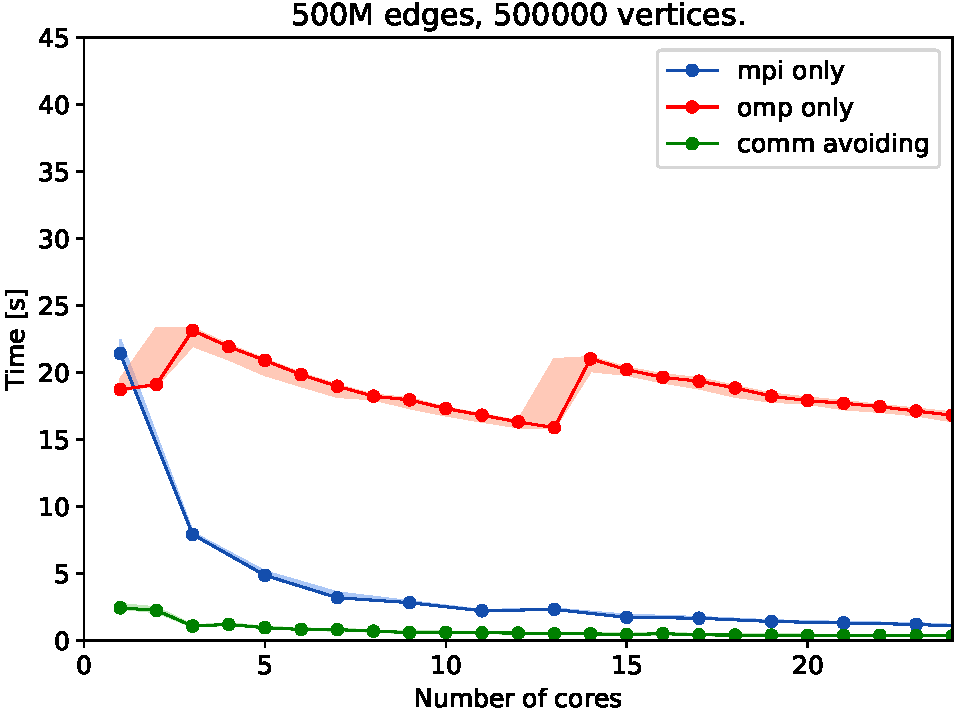
\includegraphics[width=\textwidth]{data/50000our_impl}
\subcaption{$5\times10^{5}$ vertices}
\label{fig:mpi_omp_commavoiding_euler_1}
\end{subfigure}

\begin{subfigure}[c]{\fsize}
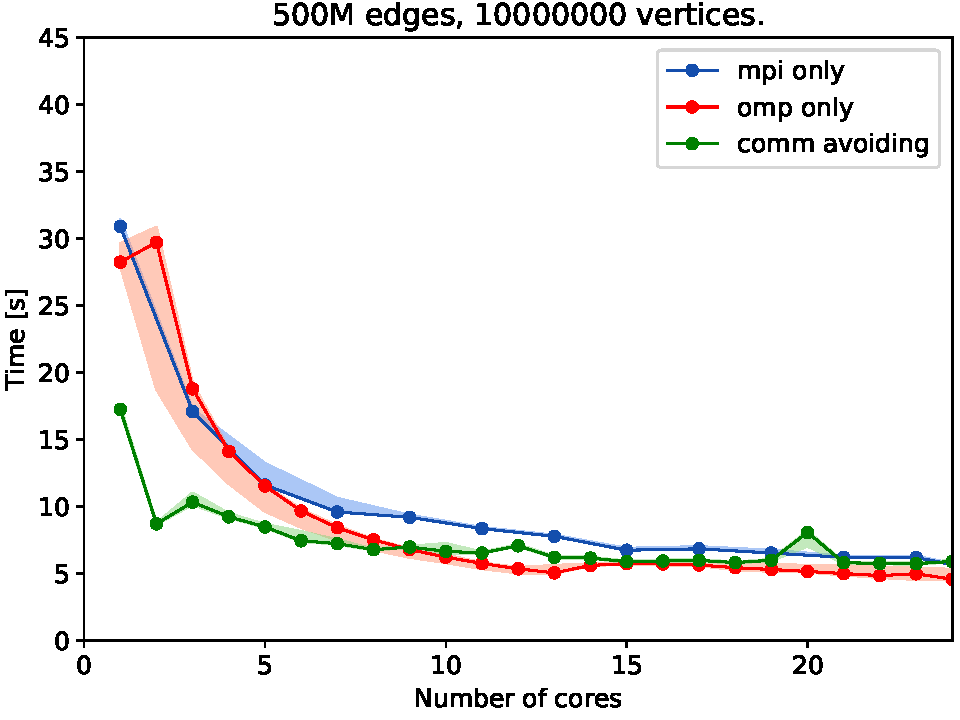
\includegraphics[width=\textwidth]{data/10000our_impl}
\subcaption{$10^{7}$ vertices}
\label{fig:mpi_omp_commavoiding_euler_2}
\end{subfigure}

\begin{subfigure}[c]{\fsize}
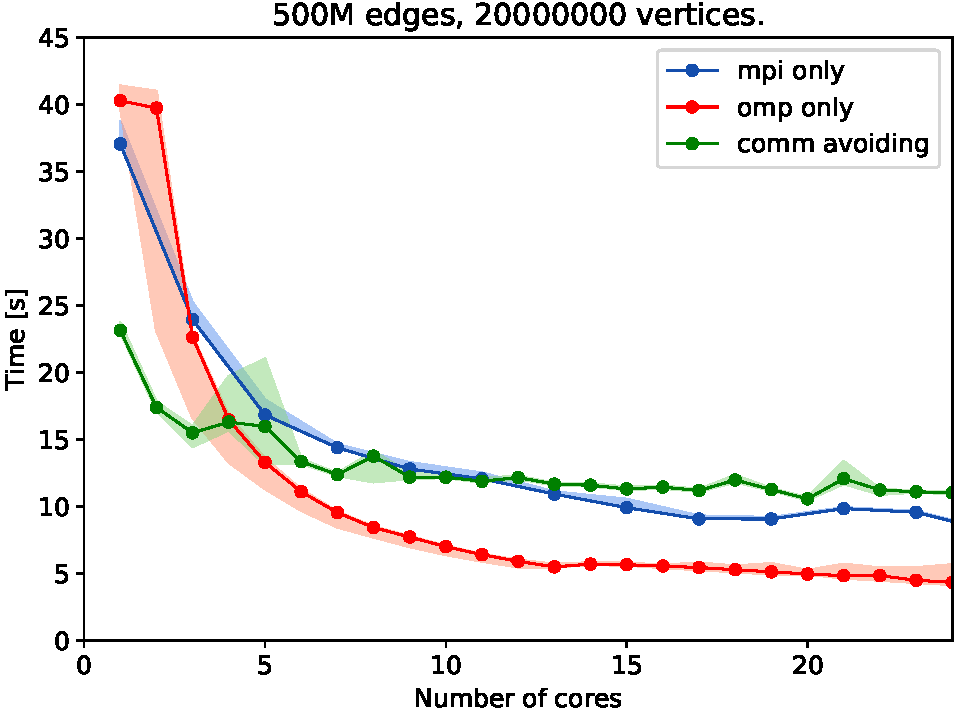
\includegraphics[width=\textwidth]{data/20000our_impl}
\subcaption{$2\times10^{7}$ vertices}
\label{fig:mpi_omp_commavoiding_euler_3}
\end{subfigure}

\caption{Comparison of the total runtime of our algorithm with the communication avoiding algorithm
\cite{comm_avoiding} over three different graphs each with $5\times10^{8}$ edges and $5\times10^5,
1\times10^7, 2\times10^7$ vertices. The experiment was run on the Euler
cluster.}
\label{fig:mpi_omp_commavoiding_euler}
\end{figure}

The results in \autoref{fig:mpi_omp_commavoiding_euler} show our algorithm compared with the
communication avoiding algorithm \cite{comm_avoiding} on three different graphs with the same
number of edges but different densities. Our algorithm was run in MPI and OMP only mode.\\
\autoref{fig:mpi_omp_commavoiding_euler_1} shows the MPI version outperforming the OMP version
on the densest graph. This can be explained by the combination of two effects. The first is that a 
dense graph results in more contention between the OMP threads during the
edge contractions. The second is that the reduction scales linearly with the number of vertices. 
Since the number of vertices is comparatively low in a dense graph the
reduction is fast. For the OMP version we further observe a significant increase in total
compute time from one to two cores and from 12 to 13 cores. The first jump can be explained by the
initial overhead of doing the computation in parallel. Since a single CPU on Euler has 12 cores the
second jump is a result of  the cache coherency protocol being slow across multiple CPUs.\\
The results in \autoref{fig:mpi_omp_commavoiding_euler_2} and
\autoref{fig:mpi_omp_commavoiding_euler_3} were obtained using sparser graphs compared to
\autoref{fig:mpi_omp_commavoiding_euler_1}. Here, for a large number of cores, the OMP version
is clearly faster than the MPI version. \autoref{fig:mpi_omp_commavoiding_euler} shows a trend
of the OMP version speeding up as the graph becomes sparser, while the MPI version slows
down. The OMP version's speed up can be explained by less contention between the OMP
threads due to the sparser graph. The MPI version's slow down is the result of the increased
reduction time due to the larger number of vertices.\\
The results in \autoref{fig:mpi_omp_commavoiding_euler} show the communication avoiding algorithm
scaling badly with the number of cores. This is expected since the edge contractions are computed
on a single node. Since our algorithm does to scale with the number of cores up
to some point we manage to outperform the communication avoiding algorithm on each graph.


%
%\mypar{Mixing MPI and OMP}
%
%\begin{figure}[H]
%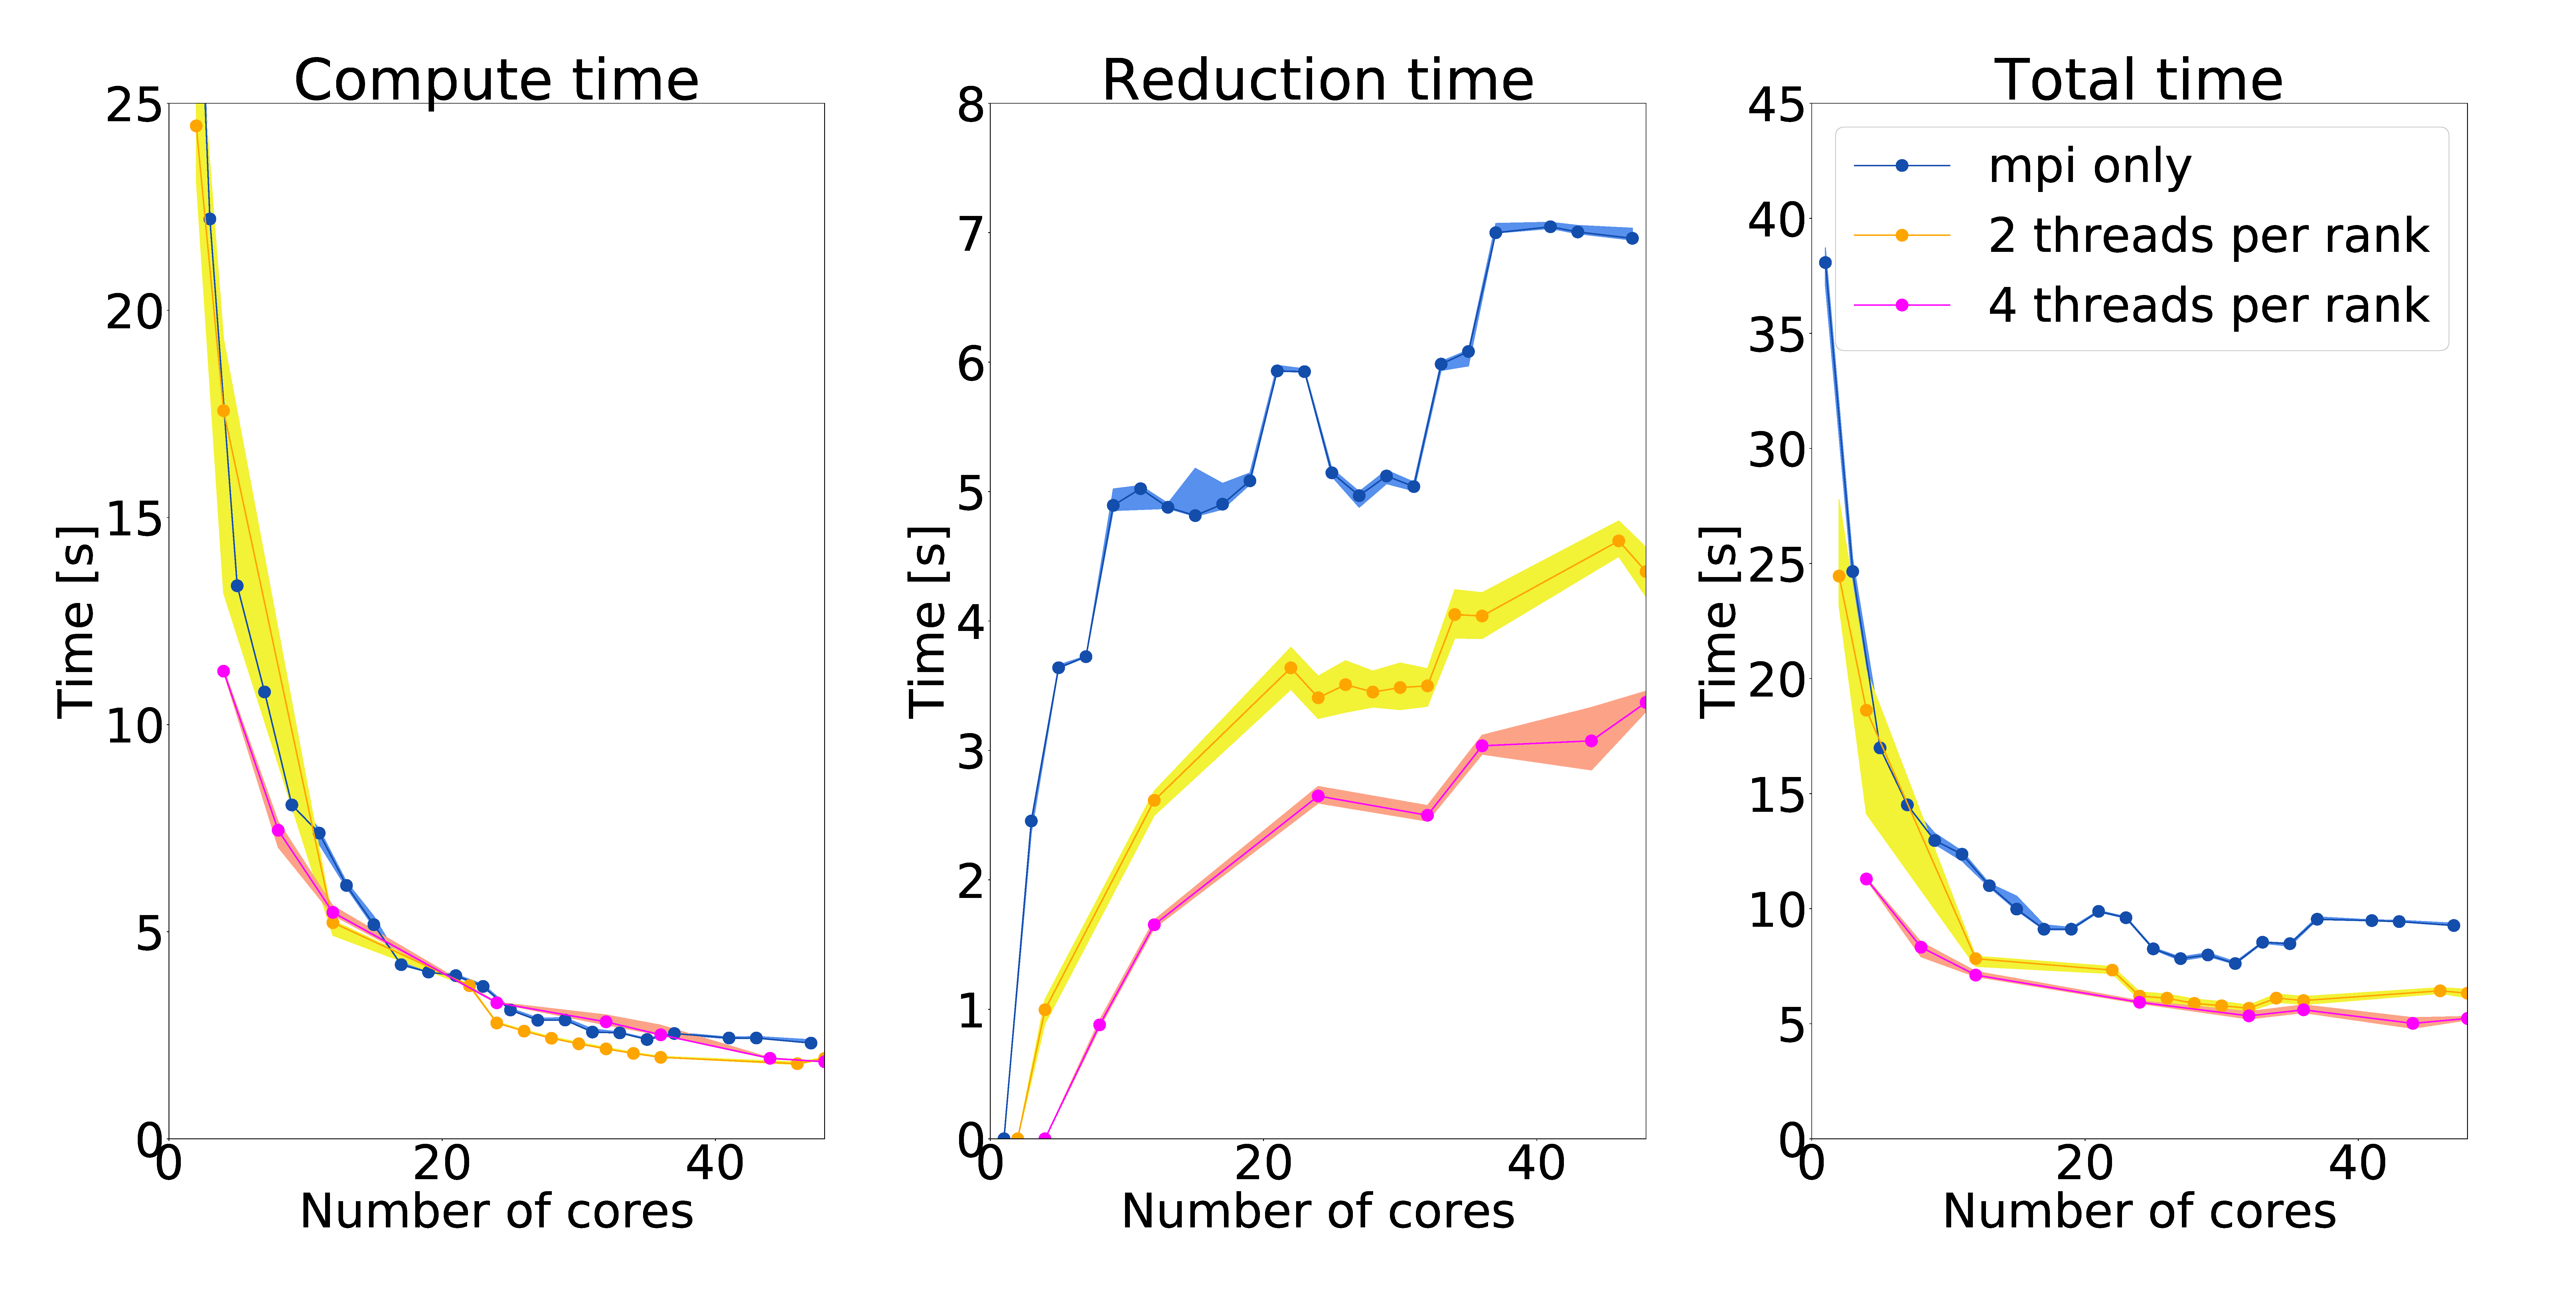
\includegraphics[width=0.5\textwidth]{plots/20000mpi_mixtures_with_everything}
%\subcaption{$2\times10^{7}$ vertices}
%\caption{Total runtime breakdown on graph with $5\times10^{8}$ edges and $2\times10^{7}$ vertices.
%The experiment was run on the Euler cluster.}
%\label{fig:mixed_euler}
%\end{figure}
%
%To further investigate the distinct difference between the MPI only and the OMP only version the
%algorithm was tested using a mixture of MPI and OMP.
%\autoref{fig:mixed_euler} shows the compute time being largely independent of the mixture. This is
%a consequence of the graphs sparsity which results in low contention between the OMP threads. The
%reduction time, however, wildly differs for the different mixtures. For each mixture it increases
%logarithmically with the number of MPI ranks. This results in the algorithm's performance
%decreasing as less OMP threads per MPI rank are used.


\mypar{Results on Piz Daint}

\begin{figure}
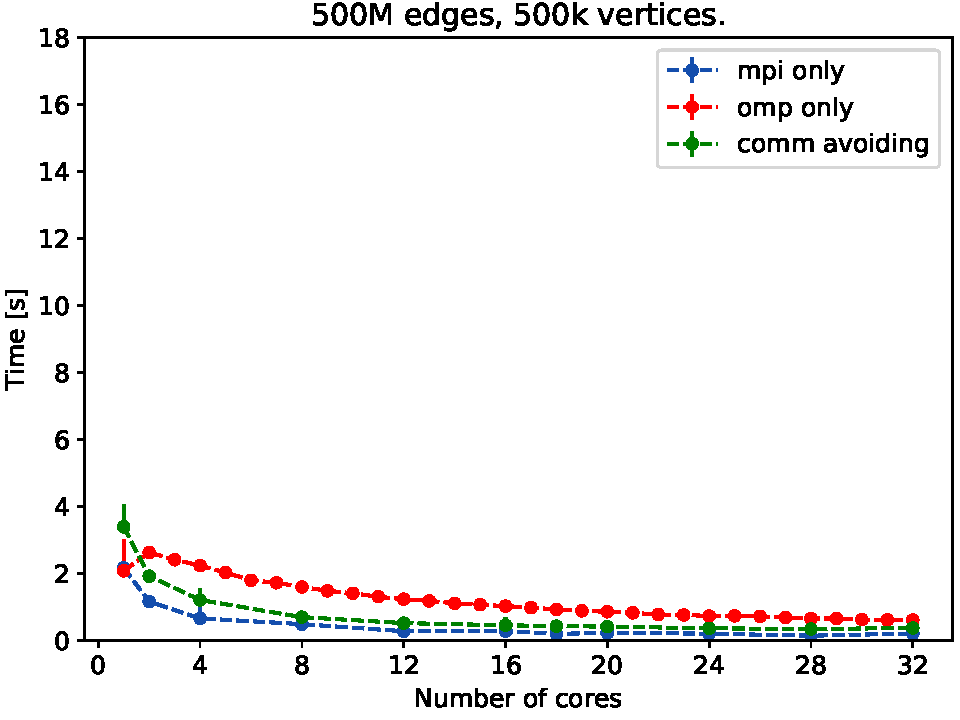
\includegraphics[width=\fsize]{data/plot_vertices_500k.pdf}
\caption{Piz Daint results on graph with $5\times10^8$ edges and $5\times10^5$ vertices.}
\label{fig:mpi_omp_commavoiding_daint_1}
\end{figure}

\begin{figure}
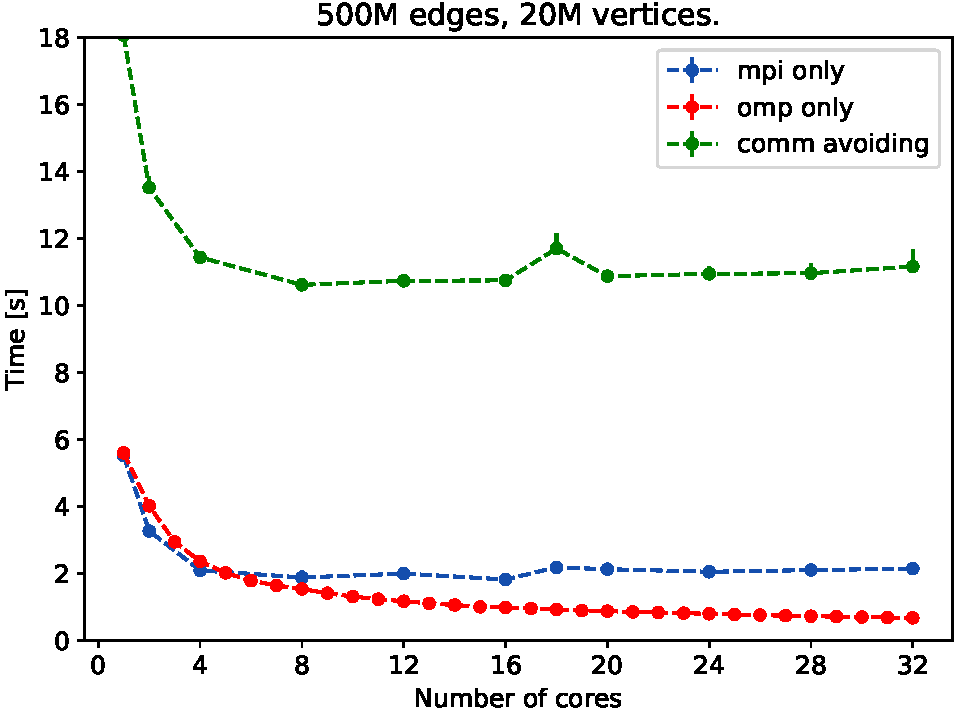
\includegraphics[width=\fsize]{data/plot_vertices_20M.pdf}
\caption{Piz Daint results on graph with $5\times10^8$ edges and $2\times10^7$ vertices.}
\label{fig:mixed_daint}
\end{figure}

Additionally we tested our algorithm on the Piz Daint cluster. The graphs used were the same as in 
the experiments run on Euler. We will now discuss interesting differences in the results.\\
\autoref{fig:mpi_omp_commavoiding_daint_1} shows the results for the densest graph on Piz Daint. 
The OMP version behaves differently compared to Euler. We still observe a decrease in performance 
when going from one to two cores. The decrease is not as severe as on Euler. The performance 
decrease as we go from one to multiple CPUs is no longer present. This can be explained by Daint's 
cache coherency protocol being more efficient, especially across multiple CPUs.
\autoref{fig:mixed_daint} shows the Piz Daint results for different mixtures of MPI and OMP on the 
sparsest graph. As on Euler, we do see the OMP version performing best for a large number of cores. 
For all versions, except the OMP version, we can clearly see the effect the number of reduction 
steps has on the runtime. It is most noticeable as we go from 16 to 18 cores. Here each version has 
to perform an additional reduction step which results in the increased runtime.





\mypar{Speedups}

\begin{figure}[H]
\begin{subfigure}[c]{\fsize}
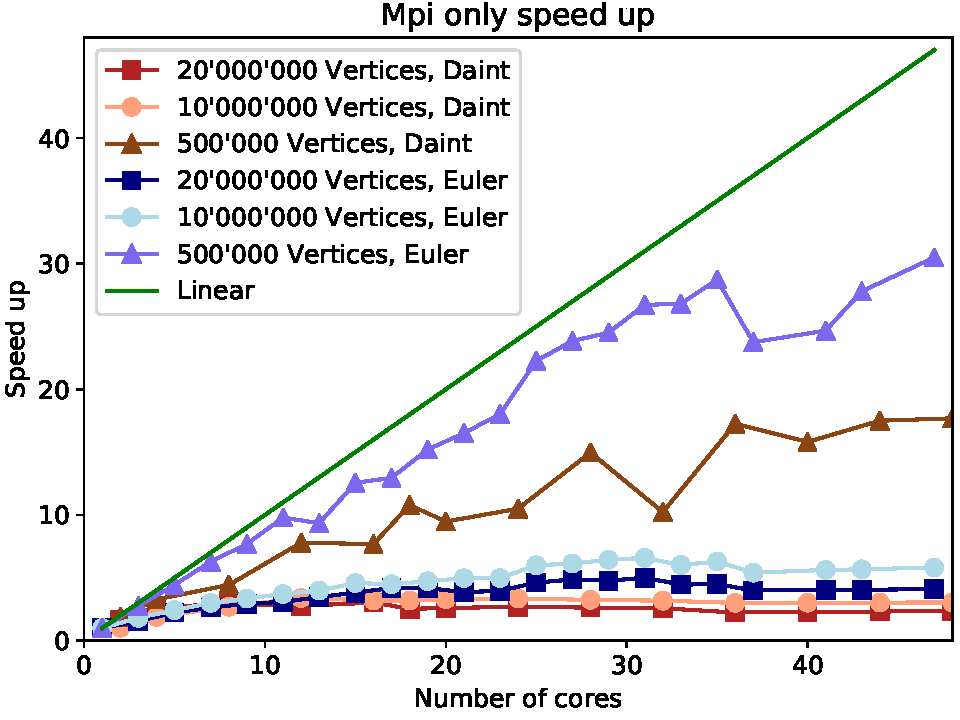
\includegraphics[width=\textwidth]{data/mpi_speedup_with_ref}
\subcaption{MPI only}
\label{fig:speedup_mpi}
\end{subfigure}
\begin{subfigure}[c]{\fsize}
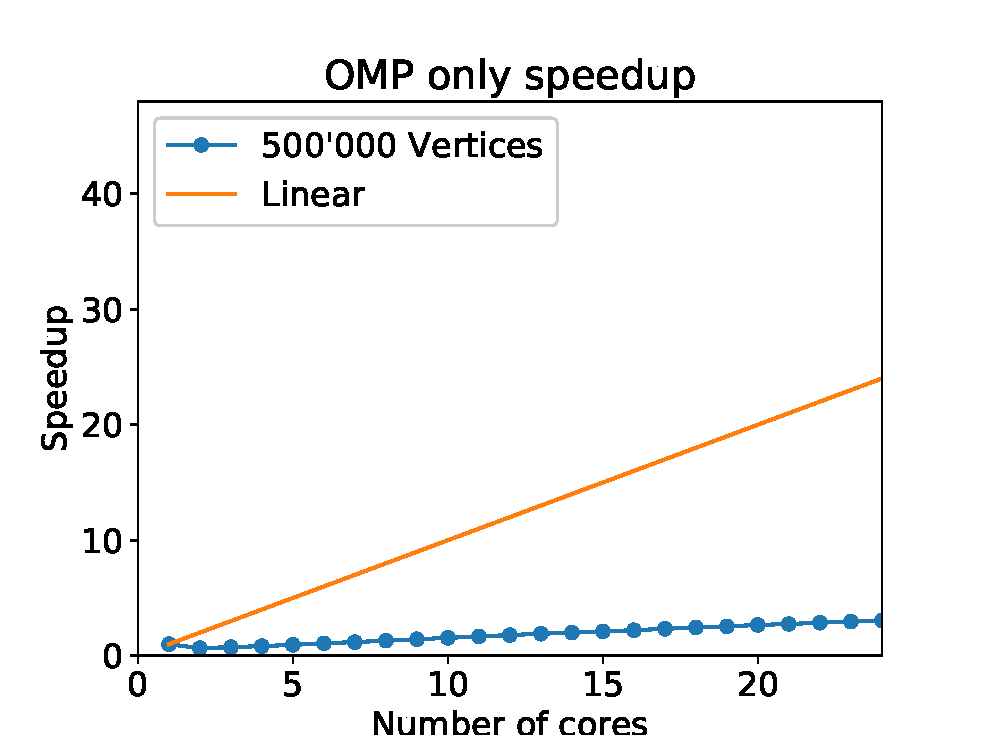
\includegraphics[width=\textwidth]{data/omp_speedup_with_ref}
\subcaption{OMP only}
\label{fig:speedup_omp}
\end{subfigure}
\caption{Speedup of MPI only and OMP only version on three different graphs each with
$5\times10^{8}$ edges.}
\label{fig:speedup}
\end{figure}

\autoref{fig:speedup} shows the measured speed up of the MPI and OMP version. As one
would expect from the results discussed previously the MPI version achieves better scaling on dense 
graphs while the OMP version scales better on sparse graphs.\\
We can also see that our algorithm achieves better scaling on Euler for the MPI version. The reason 
our algorithm scales better on Euler is that the single core performance is lower on Euler compared 
to Daint. This means that the edge contractions dominate the runtime for longer before the 
reduction step starts to be an issue.\\
For the OMP version the discrepancy in the speed ups can be explained by the differences in the 
shared memory architecture.



%Here you evaluate your work using experiments. You start again with a
%very short summary of the section. The typical structure follows.
%
%\mypar{Experimental setup} Specify the platform (processor, frequency, maybe OS, maybe cache sizes)
%as well as the compiler, version, and flags used. If your work is about performance,
%I strongly recommend that you play with optimization flags and consider also icc for additional potential speedup.
%
%Then explain what kind of benchmarks you ran. The idea is to give enough information so the experiments are reproducible by somebody else on his or her code.
%For sorting you would talk about the input sizes. For a tool that performs NUMA optimization, you would specify the programs you ran.

\mypar{Results}
%Next divide the experiments into classes, one paragraph for each. In each class of experiments you typically pursue one questions that then is answered by a suitable plot or plots. For example, first you may want to investigate the performance behavior with changing input size, then how your code compares to external benchmarks.
%
%For some tips on benchmarking including how to create a decent viewgraph see pages 22--27 in \cite{Pueschel:10}.

%{\bf Comments:}
%\begin{itemize}
%\item Create very readable, attractive plots (do 1 column, not 2 column plots
%for this report) with readable font size. However, the font size should also not be too large; typically it is smaller than the text font size.
%An example is in Fig.~\ref{fftperf} (of course you can have a different style).
%\item Every plot answers a question. You state this question and extract the
%answer from the plot in its discussion.
%\item Every plot should be referenced and discussed.
%\end{itemize}

%\begin{figure}\centering
%  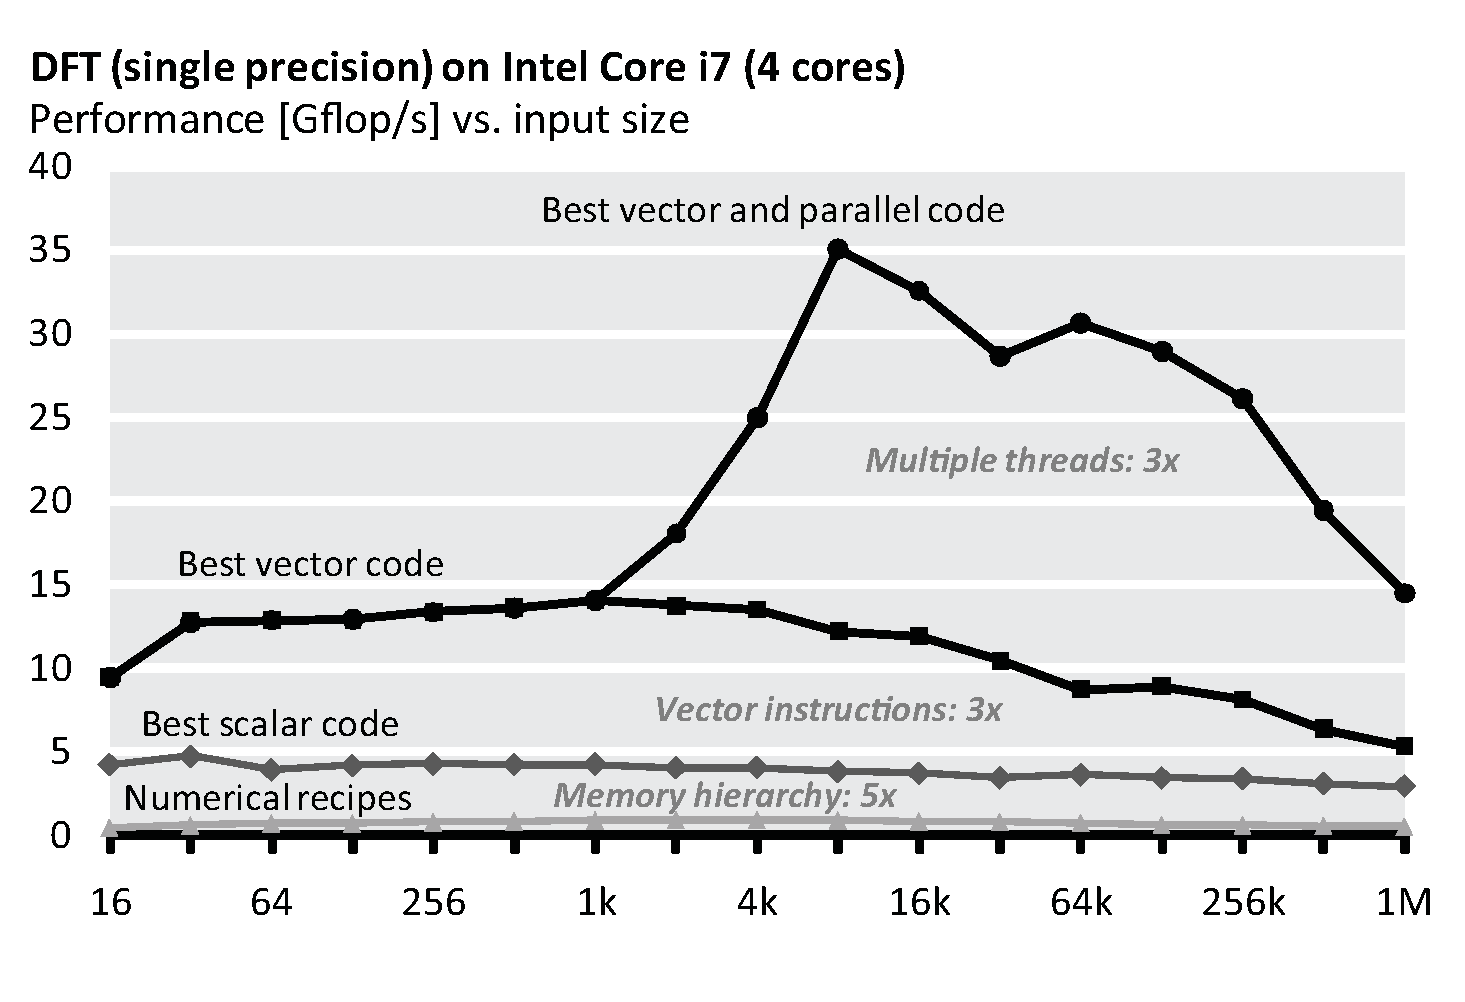
\includegraphics[scale=0.33]{dft-performance.eps}
%  \caption{Performance of four single precision implementations of the
%  discrete Fourier transform. The operations count is roughly the
%  same. The labels in this plot are maybe a little bit too small.\label{fftperf}}
%\end{figure}

\section{Conclusions}

The proposed algorithm manages to take advantage of the parallelism available within shared memory units while avoiding excessive communication between them. By choosing the right number of OMP threads per MPI rank the algorithm achieves good scaling across a variety of graphs. While on dense graphs the \replaced[id=R]{c}{C}ommunication \replaced[id=R]{a}{A}voiding algorithm \cite{comm_avoiding} yields better results, it is outperformed by our algorithm on sparser graphs. 

%Here you need to summarize what you did and why this is
%important. {\em Do not take the abstract} and put it in the past
%tense. Remember, now the reader has (hopefully) read the report, so it
%is a very different situation from the abstract. Try to highlight
%important results and say the things you really want to get across
%such as high-level statements (e.g., we believe that .... is the right
%approach to .... Even though we only considered x, the
%.... technique should be applicable ....) You can also formulate next
%steps if you want. Be brief. After the conclusions there are only the references.

\section{Future Work}

The main drawback of our algorithm is the reduction steps runtime of $O\left(n \cdot log\left(p\right)\right)$, where $p$ is the number of MPI ranks and $n$ is the number of vertices. For a large number of MPI ranks the $log\left(p\right)$ factor becomes a problem.\\
One approach to solve this problem is trying to reduce the reductions "height" of $log\left(p\right)$. In our algorithm this is done by using a mixture of OMP and MPI which reduces the number of MPI ranks. Since OMP does not scale well once the number of OMP threads exceeds the number of cores per CPU this approach is only viable up to a limited number of cores.\\
Another approach would be reducing the work $n$ done in each reduction step. Due to time constraints we were unable to investigate this approach. One could imagine a more efficient hook tree representation solving this problem.\\
\\
Another drawback of our algorithm is that in order to achieve satisfying performance one needs to find the right mixture of MPI and OMP. While we analysed the behaviour of different mixtures on graphs with varying density we did not come up with an a priori scheme to determine the right mixture. A good heuristic or even a scheme to find the optimal mixture would be worth exploring.

%Here we provide some further tips.

%\mypar{Further general guidelines}
%
%\begin{itemize}
%\item For short papers, to save space, I use paragraph titles instead of
%subsections, as shown in the introduction.
%
%\item It is generally a good idea to break sections into such smaller
%units for readability and since it helps you to (visually) structure the story.
%
%\item The above section titles should be adapted to more precisely
%reflect what you do.
%
%\item Each section should be started with a very
%short summary of what the reader can expect in this section. Nothing
%more awkward as when the story starts and one does not know what the
%direction is or the goal.
%
%\item Make sure you define every acronym you use, no matter how
%convinced you are the reader knows it.
%
%\item Always spell-check before you submit (to us in this case).
%
%\item Be picky. When writing a paper you should always strive for very
%high quality. Many people may read it and the quality makes a big difference.
%In this class, the quality is part of the grade.
%
%\item Books helping you to write better: \cite{Higham:98} and \cite{Strunk:00}.
%
%\item Conversion to pdf (latex users only):
%
%dvips -o conference.ps -t letter -Ppdf -G0 conference.dvi
%
%and then
%
%ps2pdf conference.ps
%\end{itemize}
%
%\mypar{Graphics} For plots that are not images {\em never} generate the bitmap formats
%jpeg, gif, bmp, tif. Use eps, which means encapsulate postscript. It is
%scalable since it is a vector graphic description of your graph. E.g.,
%from Matlab, you can export to eps.
%
%The format pdf is also fine for plots (you need pdflatex then), but only if the plot was never before in the format
%jpeg, gif, bmp, tif.


% References should be produced using the bibtex program from suitable
% BiBTeX files (here: bibl_conf). The IEEEbib.bst bibliography
% style file from IEEE produces unsorted bibliography list.
% -------------------------------------------------------------------------
\bibliographystyle{IEEEbib}
\bibliography{bibl_conf}

\end{document}

